% Ideia básica dos algorítmos (Coesão léxica ) como **presuposto básico**

%Os principais algoritmos de segmentação textual assumem o pressuposto que um segmento pode ser identificado e delimitado pela análise de seu vocabulário

Os principais algoritmos de segmentação textual baseiam-se na ideia de coesão léxica entre assuntos. Isto é, a mudança de tópicos é acompanhada de uma proporcional mudança de vocabulário. A partir disso, vários algoritmos foram propostos. Dessa forma, assumem o pressuposto que um segmento pode ser identificado e delimitado pela análise das palavras que o compõe.

% Porque cosine
% vetores de frencia para cada sentença que serão comparados com cosine
Uma vez que coesão léxica é pressuposto básico da maioria dos algoritmos, o cálculo da similaridade entre textos e fundamental. Uma medida de similidade frequentemente utilizada é a \textit{cosine}, a qual pode ser vista na equação~\ref{equ:cosine}, sendo $f_{x,j}$ a frequência da palavra $j$ na sentença $x$ e $f_{y,j}$ sendo a frequência da palavra $j$ na sentença $y$.


\begin{equation}
Sim(x,y) = \frac
{\Sigma_j f_{x,j} \times f_{y,j}}
{\sqrt{\Sigma_j f^2_{x,j} \times \Sigma f^2_{x,j}}}
\label{equ:cosine}
\end{equation}




% A coesão léxica é um termômetro para as mudanças de tópicos, e portanto, um indicador para quebras de segmento.

% Nesse artigo, os principais serão analisados na perspectiva de atas de reunião.


% Os entre os principais trabalhos relacionados a segmentação textual estão o \textit{TextTiling} e o \textit{C99}


%%%%%%%%%%%%%%%%%%%%%%%%%%%%%%%%%%%%%%%%%%%%%%%
%%%              TextTiling                 %%%
%%%%%%%%%%%%%%%%%%%%%%%%%%%%%%%%%%%%%%%%%%%%%%%

Entre os trabalhos mais influentes podemos citar o \textit{TextTiling}~\cite{Hearst1994} proposto por Hearst. Ela propõe um algoritmo baseado em janelas deslizantes, onde para cada candidato a limite, analisa-se o texto circundante. Um limite ou quebra se segmento é identificado quando a similaridade entres os blocos apresenta uma queda considerável.


Ela propõe um algoritmo baseado em janelas deslizante, para analisar blocos de texto adjacentes e identificar os limites com base nas similaridades dos blocos.

O algoritmo recebe uma lista de candidatos a limite, usualmente finais de parágrafo ou finais de sentenças. Para cada posição candidata são construídos 2 blocos, um contendo sentenças que a precedem e outro com as que a sucedem. O tamanho desses blocos é um parâmetro a ser fornecido ao algoritmo e determina o tamanho mínimo de um segmento.
%
Em seguida, os blocos de texto são representados por vetores que contém as frequências de suas palavras. Então, usa-se \textit{cosini} (equação~\ref{equ:cosine}) para calcular a similaridade entre os blocos.

Finalmente, os limites são identificados sempre que a similaridade entre blocos adjacentes entre cada candidato ultrapassa um determinado \textit{threshold}

Apresenta baixa complexidade computacional, devido a simplicidade do algoritmo e baixa eficiência quando comparado a outros métodos mais sofisticados como mostrando em~\cite{Choi2000, Kern2009167}.




% Citar o [Kern] como trabalho que extende o TexTiling. Ele usa _inner_ e _outter_ _similarity_. Usa Term Weighting também?



%%%%%%%%%%%%%%%%%%%%%%%%%%%%%%%%%%%%%%%%%%%%%%%
%%%                  C99                    %%%
%%%%%%%%%%%%%%%%%%%%%%%%%%%%%%%%%%%%%%%%%%%%%%%

Choi \cite{Choi2000} apresenta um trabalho que usa \textit{cosine}, a qual é exibida na equação~\ref{equ:cosine}, como medida similaridade e apresenta um esquema de ranking em seu algoritmo, o \textit{C99}. 
%
Embora muitos dos melhores trabalho utilizarem matrizes de similaridades, o autor traz obervações.
%
Ele aponta que para pequenos segmentos, o cálculo de suas similaridades não é confiável. Pois uma ocorrência adicional de uma palavra causa um impacto desproporcional no cálculo.
%
Além disso, o estilo da escrita pode não ser constante em todo o texto. Choi sugere que, por exemplo, textos iniciais dedicados a introdução costumam apresentar menor coesão do que trechos dedicados a um tópico específico. 
%

Portanto comparar a similaridade entre trechos de diferentes regiões, não é apropriado.
% Complexidade O(n²)
Devido a isso, as similaridades não podem ser comparadas em valores absolutos,  então, o autor apresenta um esquema de ranking para contornar esse problema.
%



Cada valor na matriz de similaridade é substituído por seu ranking local. Onde ranking é o número de elementos vizinhos com similaridade menor, o qual e calculado com a equação~\ref{equ:ranklocal}. Um exemplo é mostrado na Figura \ref{fig:exemplomatrixrank} abaixo.



  \begin{figure}[!h]

	\centering
	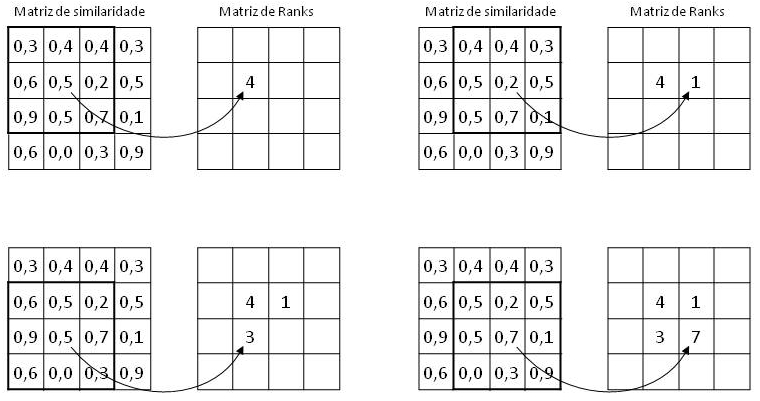
\includegraphics[width=0.45\textwidth]{exemplo-matrix-rank-noborder.jpg}
	\caption{Exemplo de construção de uma matriz de rank}
	\label{fig:exemplomatrixrank}

  \end{figure}




\begin{equation}
r(x,y) = \frac
{Numero\ de\ elementos\ com\ similaridade\ menor}
{Numero\ de\ elementos\ examinados}
\label{equ:ranklocal}
\end{equation}


% Clustering Reynar maximization
	
	Finalmente, na etapa de \textit{clustering}, Choi utiliza um método baseado no algoritmo de maximização de Reynar~\cite{reynar} para identificar os limites entre os segmentos.




Semelhante a esse trabalho, outras abordagens foram propostas como ...

\cite{Banerjee200657} faz uma adaptação do \textit{TextTiling} ao contexto das conversas em reuniões com múltiplos participantes.  


